\documentclass[9pt,a4paper,landscape]{article}
\input{template_cheatsheet}
\usepackage{polyglossia}
\setdefaultlanguage{sanskrit}
\setotherlanguage{english}

\usepackage{fontspec}
\setmainfont{Segoe UI}

% Devanagari Fonts
\newfontfamily\devanagarifont[Script=Devanagari]{Nakula}
\newfontfamily\devanagarifontsf[Script=Devanagari]{Nakula}
\newfontfamily\devanagarifonttt[Script=Devanagari]{Nakula}
\newfontfamily\devtransl[Mapping=DevRom]{Segoe UI}


\graphicspath{{images/}}


\begin{document}
\footnotesize


\begin{center}
\Large{\textbf{YogaSutra Seminar 1: Introduction}}  

\small{\textbf{Yogesh Haribhau Kulkarni}}  
\end{center}

\begin{multicols}{2}
\section[Intro]{Introduction}
\input{yogsutra_intro}

\section[End]{Towards End}
\input{yogsutra_glance}
%%%%%%%%%%%%%%%%%%%%%%%%%%%%%%%%%%%%%%%%%%%%%%%%%%%%%%%%%%%%%%%%%%%%%%%%%%%%%%%%%%
\begin{frame}[fragile]\frametitle{}
\begin{center}
{\Large References}
\end{center}
\end{frame}


%%%%%%%%%%%%%%%%%%%%%%%%%%%%%%%%%%%%%%%%%%%%%%%%%%%%%%%%%%%
\begin{frame}[fragile]\frametitle{References}

Many publicly available sources have been used in the preparation of this content. Some of the salient ones are listed below:

	\begin{itemize}
	\item Patanjali Yog Sutra https://patanjaliyogasutra.in/
	\item Yoga Sutra Study https://yogasutrastudy.info/
		\begin{itemize}
		\item [HA]: Hariharananda Aranya
		\item [IT]: I. K. Taimni
		\item [VH]: Vyasa Houston
		\item [BM]: Barbara Miller
		\item [SS]: Swami Satchidananda
		\item [SP]: Swami Prabhavananda
		\item [SV]: Swami Vivekananda
		\end{itemize}
	\item Prof. Edwin Bryant — \emph{The Yoga Sutras of Patanjali} (book + lectures)
	\item Dr. Ananda Balayogi Bhavanani — \emph{An Overview of the Yoga Sutras}, Integral Yoga Magazine
	\item Nancy Wile — \emph{The Yoga Sutras} (Yoga Teacher Training manual), Yoga Education Institute, 2014
	\item Krishnamurthy Ramakrishnan — \emph{Yoga Sutras for Daily Life}, LinkedIn Newsletter
	\item Wikipedia — \emph{Yoga Sutras of Patanjali}
	\item योग सूत्र का परिचय | Yoga Sutras of Patanjali | Yoga Sutras For QCI, UGC NET, Yoga All Exams - YouTube
	\item Patanjali Yoga Sutra Dr Mrudula Chaudhari
	\item Patanjali Yoga Sutras | Explanation by Anandmurti Gurumaa Gurumaa Ashram Verified
	\item Indica Course https://indica.courses/enroll/prof-m-a-narasimhan/maharshi-patanjali-yogasutras-learn-recite-ii/
	\item Swami J Patanjali Yoga Sutra https://swamij.com/yoga-sutras.htm
	\item Dr. Veena Londhe — \emph{An Introduction to Patanjali's Yoga Darshana}, Chinmaya Mission
	\end{itemize}

\end{frame}

%%%%%%%%%%%%%%%%%%%%%%%%%%%%%%%%%%%%%%%%%%%%%%%%%%%%%%%%%%%
\begin{frame}[fragile]\frametitle{Youtube Channels}



	\begin{itemize}
	\item Patanjali Yoga Sutras - English Yogic Gurukul - Anvita Dixit · Podcast
	\item Patanjali Yoga Sutras | Explanation by Anandmurti Gurumaa
	\item Complete Patanjali Yoga Sutras Chant with Meanings
	\item Patanjali Yoga Sutra Live Streams - The Sanskrit Channel
	\item The Sankrit Channel - "Detailed Patanjali Yoga Sutras with Pictures - Chapter 1-2-3-4"
	\end{itemize}

\end{frame}

%%%%%%%%%%%%%%%%%%%%%%%%%%%%%%%%%%%%%%%%%%%%%%%%%%%%%%%%%%%
\begin{frame}[fragile]\frametitle{}

\begin{center}
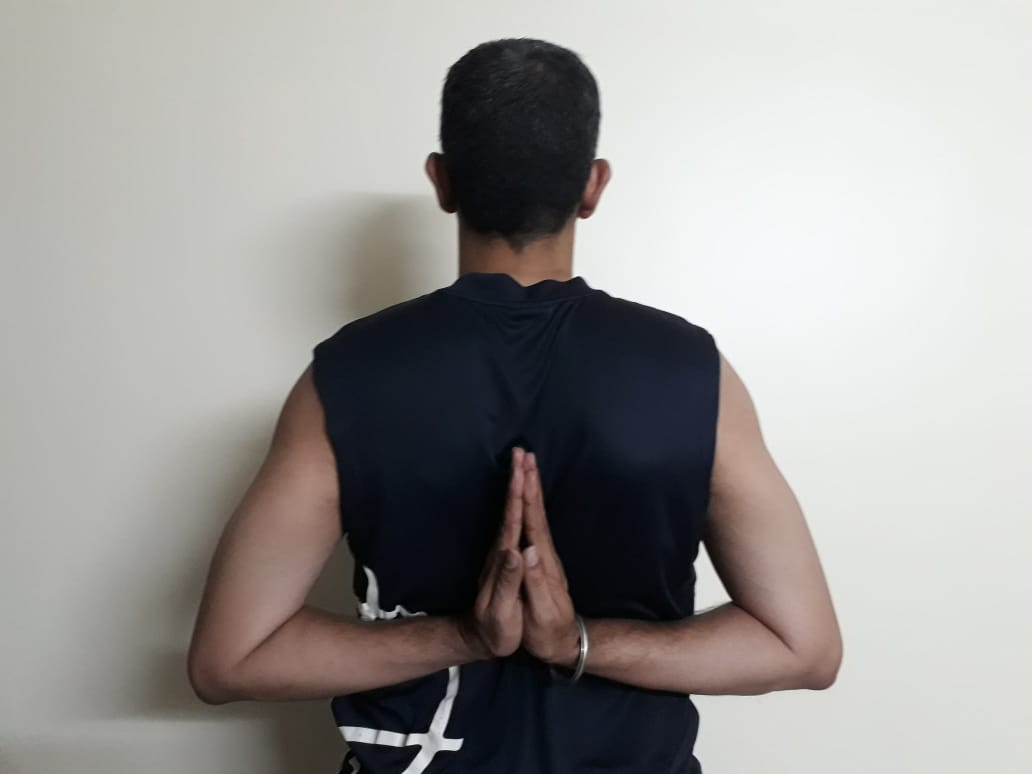
\includegraphics[width=0.8\linewidth,keepaspectratio]{my_yog_back}

Thanks धन्यवाद
\end{center}

\end{frame}

\end{multicols}

\rule{\linewidth}{0.25pt}
\scriptsize
Copyleft \textcopyleft\  Send suggestions to 
\href{http://www.yogeshkulkarni.com}{yogeshkulkarni@yahoo.com}

\end{document}
